\documentclass[11pt, a4paper]{article}

% --- UNIVERSAL PREAMBLE BLOCK ---
\usepackage[a4paper, top=1cm, bottom=1cm, left=1cm, right=1cm, landscape]{geometry}
\usepackage{tikz}
\usepackage{xcolor}
\usetikzlibrary{shapes.geometric, arrows.meta, positioning, fit, backgrounds, calc}

% --- UNIVERSITY OF SOUTH CAROLINA MARKETING TOOLBOX COLOR DEFINITIONS --- 
% Primary Colors 
\definecolor{UofSCGarnet}{RGB}{115, 0, 10} 
\definecolor{UofSCBlack}{RGB}{0, 0, 0} 
\definecolor{UofSCWhite}{RGB}{255, 255, 255} 

% Neutral Colors 
\definecolor{UofSC90Black}{RGB}{54, 54, 54} 
\definecolor{UofSC70Black}{RGB}{92, 92, 92} 
\definecolor{UofSC50Black}{RGB}{162, 162, 162} 
\definecolor{UofSC30Black}{RGB}{199, 199, 199} 
\definecolor{UofSC10Black}{RGB}{235, 235, 235} 
\definecolor{UofSCWarmGrey}{RGB}{103, 97, 86} 
\definecolor{UofSCSandstorm}{RGB}{255, 242, 227} 

% Accent Colors (Unused or Spare) 
\definecolor{UofSCRose}{RGB}{204, 46, 64} 
\definecolor{UofSCAtlantic}{RGB}{70, 106, 159} 
\definecolor{UofSCCongaree}{RGB}{31, 65, 77} 
\definecolor{UofSCHorseshoe}{RGB}{101, 120, 11} 
\definecolor{UofSCGrass}{RGB}{206, 211, 24} 
\definecolor{UofSCHoneycomb}{RGB}{164, 145, 55} 

% Special Use Colors 
\definecolor{UofSCDarkGarnet}{RGB}{87, 0, 8} 
\definecolor{UofSCAzalea}{RGB}{132, 66, 71}

\begin{document}
\thispagestyle{empty}

\begin{figure}[htbp]
\centering
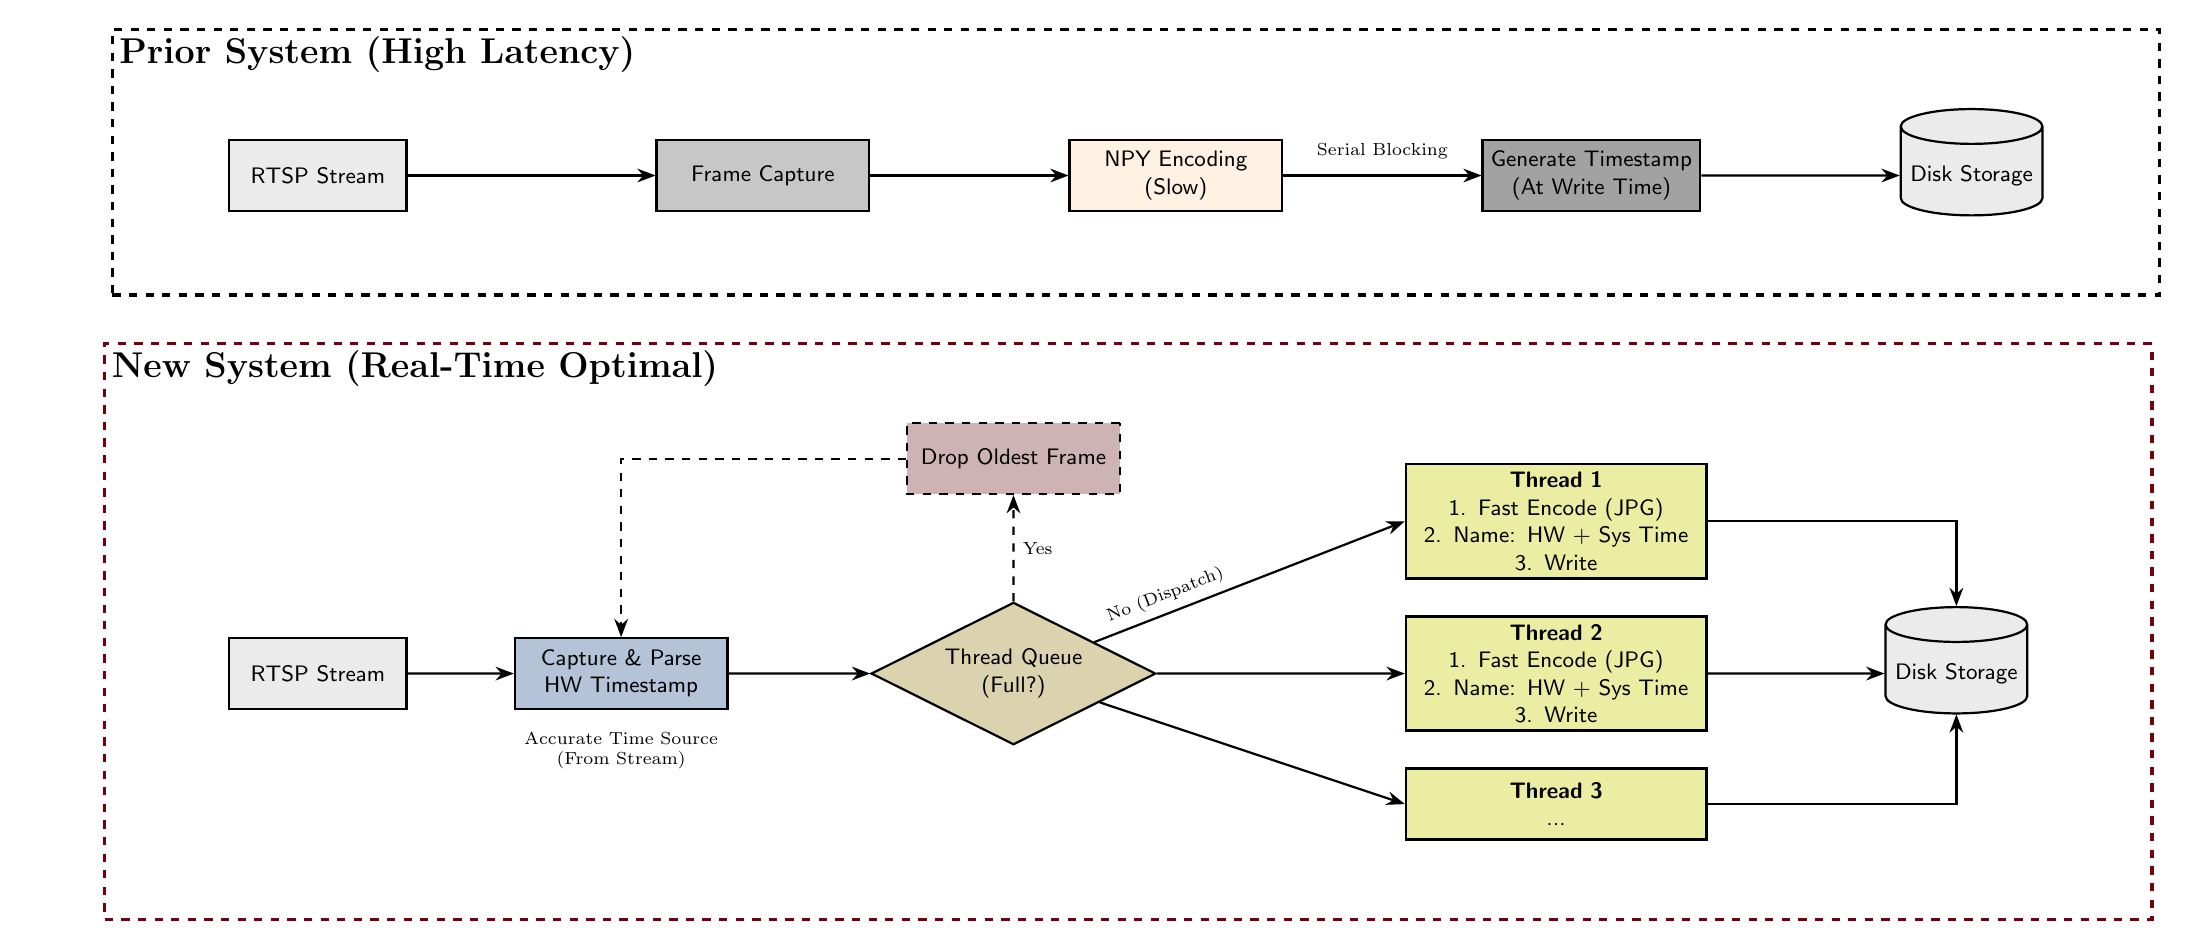
\begin{tikzpicture}[
    scale=0.9, transform shape,
    node distance=2.0cm and 2.5cm, 
    font=\small\sffamily,
    % Styles - Default fill is UofSCWhite
    startstop/.style={rectangle, thick, minimum width=2.5cm, minimum height=1cm, align=center, draw=UofSCBlack, fill=UofSCWhite, text=UofSCBlack},
    process/.style={rectangle, thick, minimum width=3cm, minimum height=1cm, align=center, draw=UofSCBlack, fill=UofSCWhite, text=UofSCBlack},
    decision/.style={diamond, thick, aspect=2, minimum width=3cm, minimum height=1cm, align=center, draw=UofSCBlack, fill=UofSCWhite, text=UofSCBlack},
    storage/.style={cylinder, thick, shape border rotate=90, aspect=0.25, minimum width=2cm, minimum height=1.5cm, align=center, draw=UofSCBlack, fill=UofSCWhite, text=UofSCBlack},
    arrow/.style={thick, ->, >=Stealth, color=UofSCBlack},
    line/.style={thick, -, color=UofSCBlack},
    labelbox/.style={rectangle, draw=none, fill=none, align=center, font=\scriptsize\itshape, text=UofSCBlack}
]

% ==========================================================================================
% PRIOR SYSTEM (Top Half)
% ==========================================================================================

% RTSP Stream - Gray Fill
\node[startstop, fill=UofSC10Black] (old_rtsp) {RTSP Stream};

% Frame Capture - Light Gray Fill
\node[process, right=3.5cm of old_rtsp, fill=UofSC30Black] (old_capture) {Frame Capture};

% NPY Encoding - Sandstorm Fill
\node[process, right=2.8cm of old_capture, fill=UofSCSandstorm] (old_encode) {NPY Encoding\\(Slow)};

% Timestamp - Medium Gray Fill
\node[process, right=2.8cm of old_encode, fill=UofSC50Black] (old_timestamp) {Generate Timestamp\\(At Write Time)};

% Disk Storage - Gray Fill
\node[storage, right=2.8cm of old_timestamp, fill=UofSC10Black] (old_disk) {Disk Storage};

% Arrows
\draw[arrow] (old_rtsp) -- (old_capture);
\draw[arrow] (old_capture) -- (old_encode);
\draw[arrow] (old_encode) -- node[midway, above=0.1cm, font=\scriptsize, text=UofSCBlack] {Serial Blocking} (old_timestamp);
\draw[arrow] (old_timestamp) -- (old_disk);

% Container for Old System
\begin{scope}[on background layer]
    \node[fit=(old_rtsp)(old_disk), draw=UofSCBlack, dashed, very thick, fill=UofSCWhite, inner sep=1.0cm, minimum width=26cm, name=old_container] {};
\end{scope}

% Title
\node[font=\Large\bfseries, text=UofSCBlack, anchor=north west] at (old_container.north west) {Prior System (High Latency)};


% ==========================================================================================
% NEW SYSTEM (Bottom Half)
% ==========================================================================================

% Position relative to the top container
% RTSP Stream - Gray Fill
\node[startstop, below=6cm of old_rtsp.south, anchor=north, fill=UofSC10Black] (new_rtsp) {RTSP Stream};

% Nodes
% Capture & Parse - Atlantic Blue Fill (Lightened)
\node[process, right=1.5cm of new_rtsp, fill=UofSCAtlantic!40] (new_capture) {Capture \& Parse\\HW Timestamp};
% Thread Queue - Honeycomb Fill (Lightened)
\node[decision, right=2cm of new_capture, align=center, fill=UofSCHoneycomb!40] (new_queue) {Thread Queue\\(Full?)};

% Drop Logic - Azalea Fill (Lightened)
\node[process, above=1.5cm of new_queue, dashed, text=UofSCBlack, fill=UofSCAzalea!40] (drop) {Drop Oldest Frame};
\draw[arrow, dashed, color=UofSCBlack] (new_queue) -- node[right, font=\scriptsize, text=UofSCBlack] {Yes} (drop);
\draw[arrow, dashed, color=UofSCBlack] (drop) -| (new_capture);

% Threads - Grass Green Fill (Lightened)
\node[process, right=3.5cm of new_queue, yshift=0cm, line width=1pt, text width=4cm, text=UofSCBlack, fill=UofSCGrass!40] (thread2) {\textbf{Thread 2}\\1. Fast Encode (JPG)\\2. Name: HW + Sys Time\\3. Write};
\node[process, above=0.5cm of thread2, line width=1pt, text width=4cm, text=UofSCBlack, fill=UofSCGrass!40] (thread1) {\textbf{Thread 1}\\1. Fast Encode (JPG)\\2. Name: HW + Sys Time\\3. Write};
\node[process, below=0.5cm of thread2, line width=1pt, text width=4cm, text=UofSCBlack, fill=UofSCGrass!40] (thread3) {\textbf{Thread 3}\\...};

% Arrows - Black
\draw[arrow, color=UofSCBlack] (new_rtsp) -- (new_capture);
\draw[arrow, color=UofSCBlack] (new_capture) -- (new_queue);
\draw[arrow, color=UofSCBlack] (new_queue) -- node[above, font=\scriptsize, sloped, near start, text=UofSCBlack] {No (Dispatch)} (thread1.west);
\draw[arrow, color=UofSCBlack] (new_queue) -- (thread2.west);
\draw[arrow, color=UofSCBlack] (new_queue) -- (thread3.west);

% Storage - Gray Fill
\node[storage, right=2.5cm of thread2, fill=UofSC10Black] (new_disk) {Disk Storage};

% Arrows from Threads to Disk - Black
\draw[arrow, color=UofSCBlack] (thread1.east) -| (new_disk);
\draw[arrow, color=UofSCBlack] (thread2.east) -- (new_disk);
\draw[arrow, color=UofSCBlack] (thread3.east) -| (new_disk);

% Annotations - Black
\node[below=0.2cm of new_capture, text width=3cm, align=center, font=\scriptsize, text=UofSCBlack] {Accurate Time Source (From Stream)};

% Container for New System
\begin{scope}[on background layer]
    % Container outline remains Garnet for distinction, internal text/arrows are Black
    \node[fit=(new_rtsp)(new_disk)(drop)(thread1)(thread3), draw=UofSCGarnet, dashed, very thick, fill=UofSCWhite, inner sep=1.0cm, minimum width=26cm, name=new_container] {};
\end{scope}

% Title moved to Top Left of the Container - Black
\node[font=\Large\bfseries, text=UofSCBlack, anchor=north west] at (new_container.north west) {New System (Real-Time Optimal)};

% Aligning the boxes
\coordinate (old_start) at (old_container.west);
\coordinate (new_start) at (new_container.west);
\path (old_start) -- (new_start) node[midway, xshift=-1cm] {};

\end{tikzpicture}
\caption{Comparison of Video Ingestion Pipelines}
\end{figure}

\end{document}